\documentclass[journal]{IEEEtran}

\usepackage{amsmath}
\usepackage{url}
\usepackage{graphicx}
\usepackage{algorithm}
\usepackage{algorithmicx}
\usepackage{algpseudocode}

\title {SOFL: Self-organizing Federated Learning Based on Multi-party Computation and Consensus Algorithm}
\author{Zhaoyang Han}


\begin{document}
\maketitle

\begin{abstract}
With the rapid development and widespread application of artificial intelligence (AI) technologies, privacy and security are attracting more attention in machine learning areas. Federated Learning (FL) is a framework based on which numerous parties can train a machine learning model cooperatively without leaking information about their data. Parties in FL send parameters of local models instead of their data to the server to protect their local data from leaking. However, researches have proven that attackers can reveal FL parties' data through the leakage of local model parameters. Therefore, secure aggregation is requisite to ensure privacy-preserving in FL frameworks. Moreover, it usually costs a lot for FL parties to securely communicate with each other. Therefore, efficiency is another problem for FL to address. In this paper, we propose a privacy-preserving FL framework based on secure multi-party computation (MPC) and simplified consensus algorithm, namely Self-organizing Federated Learning (SOFL). Our method adopts secret sharing to hide local model parameters and runs a consensus algorithm to ensure the communication is reliable, robust, and efficient.

\end{abstract}

\begin{IEEEkeywords}
    Federated Learning, Secure Aggregation, Machine Learning, Multi-party Computation, Consensus algorithm
\end{IEEEkeywords}


\section{Introduction} 
\label{sec:intro}
Smart phones and other devices in daily life are equipped with more and more powerful computing and storage abilities, which enables individual devices accumulate more and more valuable information. It facilitated a lot of rising technologies such as edge computing. Meanwhile, the accumulated data in users' devices can be used to train models for various practical purposes due to the flourish of machine learning. In traditional machine learning frameworks, data needs to be gathered in a center server in order to execute the learning process. However, most data collected by mobile devices is sensitive. Users usually refuse to send their private data to others, such as a learning center. 

Federated Learning\cite{mcmahan2016communicationefficient} is designed to address this problem. In each round, FL parties receive a global model from the server, and they train their the model based on their own data respectively. Afterwards, the partes send the parameters of their own models to the server while the server run a particular algorithm to compute the global model based on these parameters. In such frameworks, users don't need to send their data to the learning server, which can protect the privacy to some extent.

However, many researches have shown that attackers are able to infer users' data through the leaked information about the model's parameters\cite{Beyond, Leakage}. Therefore, sending parameters to the server directly is no longer secure. Secure aggregation protocols allow a group of parties who have private information to compute a function which takes these private values as parameters. Researchers paid their attention to secure aggregation for a better solution\cite{shi2011privacy,RobustAgg,Bonawitz19,Nike,PrivFL}. There are 3 primary methods to achieve privacy-preserving in secure aggregation: Differential Privacy (DP), homomorphic encryption (HE), and secure multi-party computation. DP enabled FL\cite{Bayesian,DPAnalysis,ZhuDP,geyer2017differentially,Hybrid} focuses on provides privacy-preserving while keep the accuracy of machine learning model. Since these studies did not conduct experiments with complicated machine learning models while some researches have pointed out that DP based FL will impact the accuracy of the learned model\cite{Two-Phase}, it is still a challenge to employ DP in FL. Homomorphic encryption algorithms are intuitionistic and simple to protect privacy, however they suffer from low efficiency which is hardly accecptable in FL. Blockchain-based methods\cite{DeepChain,Lu2020,On-Device} are also very promising, and the generally used consensus algorithms in them can be inspiring. Yet blockchain-based methods are still implement-unfriendly. Therefore, adopting MPC to protect users' privacy is more practical. There are many researches protecting the parameters based on MPC\cite{Practical,Two-Phase,Weighted,Hybrid}. 

Secure multi-party computation can be implemented by garbled circuits or secret sharing methods\cite{Shamir}. Garbled circuits have many limits and low effiency. Therefore, we choose to use secret sharing methods. Normally, secret sharing needs parties to exchange information among themselves. However, in federated learning frameworks, the parties are usually strange to each other, which means one party does not have the addresses of others. A party cannot communicate with other parties directly and they can only exchange information securely with the help of the server. In this case, Bonawitz etc.\cite{Practical} proposed a method about constructing secure channels among FL parties. Constructing secure channels between every pair of parties cost plenty of time, which leads to a new problem. In addition, the robustness of FL frameworks is also significant because it usually costs a lot to recover from situations that several nodes are crashed. In summary, employing traditional MPC methods in a system with large number of users is faced with a problem about efficiency and instability.

In this paper, we propose Self-organizing Federated Learning (SOFL), a novel FL framework which utilizes MPC to protects users' privacy and takes advantages of consensus algorithms to achieve high efficiency and robustness. Our model first elects some leaders, who will construct secure commnunication with other parties. Afterwards, a party only needs to exchange information with the leaders. The leaders will send the received information to the server, who helps forwarding the information to the corresponding destinations. Appointing leaders reduces the need of communications greatly and running a consensus algorithm can handle unexpected situations where a leader node or a common client is crashed. We adopted MPC protocols similar with Zhu etc\cite{Weighted}. Our model also has strong robustness based on the consensus algorithm. 

\textbf{Roadmap:} In Section~\ref{sec:back} we introduce the background of knowledge and some definitions. Next we introduce platforms of federated learning in Section~\ref{sef:related}. Section~\ref{sec:sofl} detailedly illustrates our proposed framework while describes the attack model. Evaluations for efficiency and security are stated in Section~\ref{sec:eval}, followed with experiments and results in Section~\ref{sec:exp}. Finally, we give the conclusion and future expectations in Section~\ref{sec:conc}.

\section{Background}
\label{sec:back}
In this section, we briefly introduce the concepts of key exchange, Federated Learning, multi-party computation and Consensus Algorithms, which are used in our proposed framework.

\subsection{Key Exchange}
Key exchange protocols allow several parties to share secret keys under unsafe conditions. Diffie-Hellman~\cite{DH} (DH) is a prestigious key exchange protocol. We introduce how DH protocol helps two parties to achieve agreement: suppose $a$ and $b$ want to obtain a secret key by means of DH. First they select a group $G$ of order q, and randomly choose a number $x_a$ and $x_b$ respectively. Then $a$ calculates $g_a = g^{x_a}$, where $g$ is a generator of $G$, and $b$ calculates $g_b = g^{x_b}$. $a$ sends $g_a$ to $b$, and $b$ sends $g_b$ to $a$. Finally they can calculate the shared secret $s_{ab}$ respectively:
$$ s_{ab} = g_b^{x_a}  = g_a^{x_b} = g^{x_ax_b}$$

In this scheme, only $g_a$ and $g_b$ are sent under an unsafe condition. Attackers cannot infer $s_{ab}$ from $g_a$ and $g_b$, therefore $a$ and $b$ can communicate privately by means of $s_{ab}$. DH is lightweight and efficient, and it can be expanded to multi-party versions easily in order to enable more parties to share pairwise keys.


\subsection{Federated Learning}
% Federated Learning was first proposed by McMahan and the algorithm was named FedAvg~\cite{mcmahan2016communicationefficient}. 

FL requires a number of users to jointly train a model. It usually runs for rounds. In each round, each user will train the model based on its data and get the model's parameter. Denote the $i$-th user's local parameter in the $t$-th round by $W_i^t$. When all users have trained their model in the $t$-th round, an aggregation algorithm $Agg$ will be called to compute the global model's parameter $Agg(W_1^t, W_2^t, ..., W_n^t)$, where $n$ is the total number of users. For example, weighted average was adopted as $Agg$ in FedAvg~\cite{mcmahan2016communicationefficient}. FL not only helps to protect users' privacy but also deals with the ``data in form of isolated islands'' problem for companies or institutions. Yang \emph{et al}. also categorized FL into horizontal, vertical and hybrid styles based on the fact that whether the data shares the same feature space or entities~\cite{yang2019federated}. 

Federated Learning can be generalized to two work environments:

\begin{enumerate}

    \item \textbf{Among-institutions:} In this situation, FL is usually used to help companies or other institutions solving the ``data in form of isolated islands'' problem. Generally, companies and institutions are in equal status in an FL framework. Therefore, we can suppose one party can communicate with any other one privately, i.e., P2P is already enabled in this environment.

    \item \textbf{Server based:} In this case a company or institution adopts FL to train a model based on their users' data while protecting their privacy. An FL party is a common user, which means users' communication usually needs to go through the server. With an honest-but-curious server, all information may be eavesdropped by it. Therefore, the problem with confidence is severe in such environments.

\end{enumerate}

Figure~\ref{fl_model} illustrates the structures of two environments. Executing MPC protocols and consensus algorithms are at a low price in the first environment. In the second environment, if local parameters need to be protected, we need to run some key-exchange protocols first to construct secure channels among users. One of our contributions is that we solved the problem in the second environment by building connections selectively and efficiently.


\begin{figure}[!ht]
    \centering
    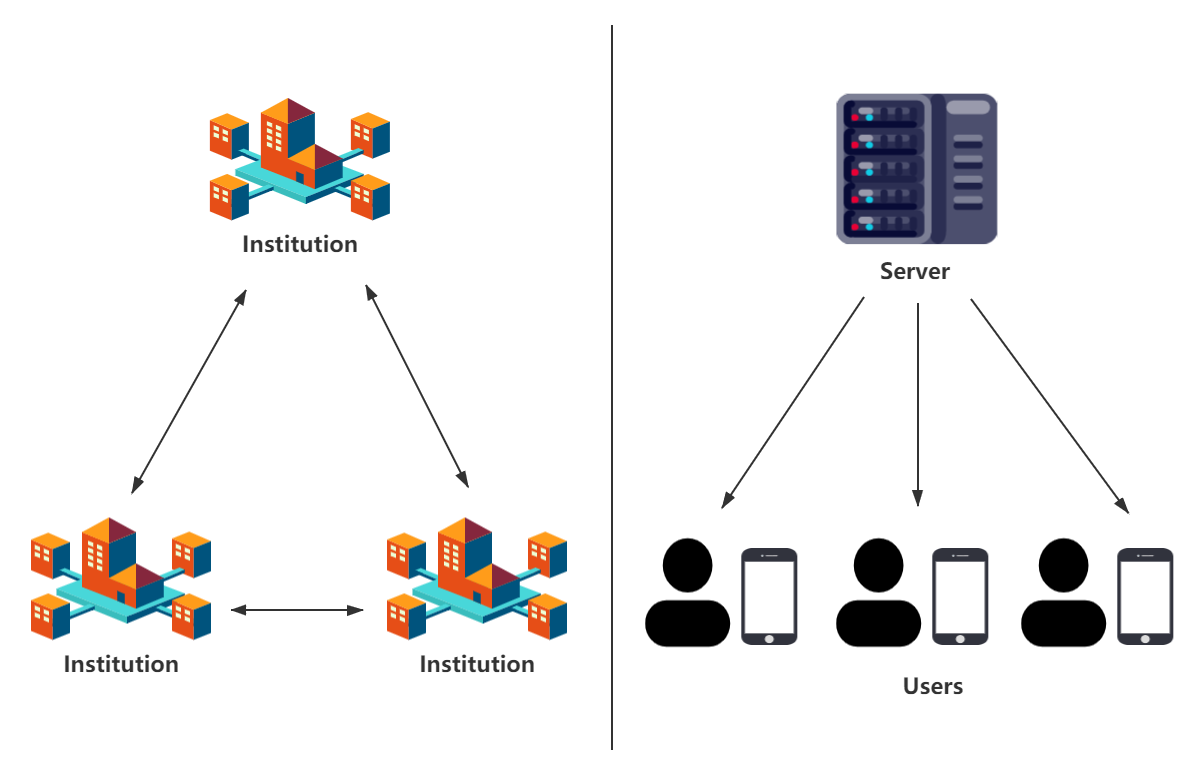
\includegraphics[width=\columnwidth]{img/fl_model.png}
    \caption{The structures of two work environments in FL. The left is the ``Among-institutions'' model where institutions can communicate with others directly, and the right is ``Server based'' model where parties exchange information in virtue of the server.}
    \label{fl_model}
\end{figure}


\subsection{Multi-party Computation}
Secure MPC is a branch of cryptography which enables several parties to compute a particular function without leaking their own data (inputs). Suppose there are $n$ parties employing MPC to compute a function $F$, and the $i^{th}$ party has its parameter $A_i$. Their goal is to compute $R = F(A_1, A_2, ..., A_n)$. MPC has the feature that participants can only obtain $R$ from the process and the party $P_i$ has no idea about parameter $A_j (j \ne i)$. This feature fits the aggregation algorithm in FL greatly.

It was first proposed by Yao to solve the millionaire problem~\cite{Yao}. Most MPC protocols depend on two cryptography technologies: secret sharing~\cite{Shamir} and oblivious transfer~\cite{OT}. MPC can be implemented with garbled circuits, multi-party circuit-based protocols or hybrid methods~\cite{mpc-sok}. It also benefits from fully homomorphic encryption (FHE) algorithms. Garbled circuits and FHE suffer from complicated design and poor efficiency. Therefore, secret sharing methods are more favored to solve the privacy-preserving problem in FL. SPDZ~\cite{SPDZ} (speedz) is a practical and secure MPC protocol introduced by Damgard \emph{et al}. It supports addition and multiplication by means of the triples~\cite{Triple}, which are generated by somewhat homomorphic encryption (SHE). Our method does not require multiplication and hence we do not need to generate the triples choose to use simple additive MPC.

A secret sharing scheme involves a secret $s$, a set of $n$ parties, and a collection $A$ of subsets of parties. Each party has its share of $s$. The secret sharing scheme ensures any subset in $A$ can reconstruct $s$~\cite{Secret-Sharing-survey}. By means of secret sharing, we can implement secure additions among parties, which is essential in our framework.


\subsection{Consensus Algorithms}
In a distributed or multi-party system, there is always a problem with consensus, i.e., in such systems parties always need to achieve agreement on a certain value. This could be difficult without any strategy because different parties may be in different statuses and have multifarious matters. Consensus algorithms are adopted to address such problems. It is widely used in blockchain and various famous areas.

Paxos was the first consensus algorithm introduced by Lamport~\cite{Paxos}. It is used in a lot of famous projects such as Ceph~\cite{Ceph}. Raft is a modification of Paxos which is more industrial-friendly~\cite{Raft}. It contains two phases: leader election and log replication. Parties can achieve agreements based on leaders. Considering that FL model is a semi-decentralized system, our framework can utilize Raft algorithm to select several leaders, based on which MPC protocols can be executed efficiently and robustly.


\section{Related Work}
\label{sec:related}
Homomorphic encryption based solutions are intuitively effective to solve aggregation problems, and there are many researchers tried to reduce the overhead caused by HE\cite{abs-1711-10677,BatchCrypt}. However, they still cost much time on computation compared to MPC based and DP based methods. DP based solutions have better performance than HE based solutions, and many works proved DP does not reduce the accuracy of machine learning models in some particular situations\cite{Bayesian,DPAnalysis,ZhuDP,geyer2017differentially}. Whereas these methods did not prove DP does not impact the accuracy in other more complicated and large-scale models. MPC based methods have the least computation cost but require more communications. A typical MPC federated learning model is implemented by Google\cite{Practical}. It requires pairwise key exchange among all clients, which results in enormous overhead on communication. Other researches present hybrid methods\cite{Hybrid,HybridAlpha}. These hybrid methods combine MPC with either HE or DP and make tradeoff on computation and communication.

Federated learning is more and more practical nowadays. FATE\cite{fate} is an open-source federated learning project proposed by Webank’s AI Department. It adopts both MPC and HE to implement secure aggregation, while it is still absorbing state-of-the-art methods for privacy-preserving. Pysyft\cite{pysyft} is another open-source federated learning framework presented by OpenMined. It is based on Pytorch and offers HE, DP, and MPC as alternative methods to realize privacy-preserving. However, the cost of time of Pysyft is dozens of times than pure Pytorch, which indicates that privacy-preserving methods of current federated learning platforms need to be improved.


\section{Self-organizing Federated Learning}
\label{sec:sofl}
In this section, we introduce the attack model and detailed design of the proposed framework Self-organizing Federated Learning. At first definitions of some symbols are listed below:
\begin{itemize}
    \item $\textbf{N}$: The total number of parties in FL system, and the  $i^{th}$ party is marked as $P_i$.
    \item $\textbf{S}$: The server, which is the host of federated learning and helps other parties to forward messages.
    \item $\textbf{frac}$: The fraction of users that will participate in the learning process each round.
    \item $\textbf{n}$: In each epoch, $n$ parties will be chosen to train the model. $n = N * frac$.
    \item $\textbf{N}_l$: Number of leaders elected from $N$ parties.
    \item $\textbf{L}$: The set of leaders.
    \item $\textbf{W}$: The parameters of a machine learning model. $W_i$ means the $i^{th}$ party's local parameter, and $W_{global}$ is the global model's parameter.
    \item $\textbf{C}$: The total number of training data. $C = \sum_{i=1}^nC_i$, where $C_i$ is the number of training data of the $i^{th}$ party $P_i$.
\end{itemize}

Our framework is based on FedAvg, which computes the weighted average of local parameters as the global parameter. In epoch $t+1$, the server's target is to compute the following formula:

$$W_{global}^{t+1} = \sum_{i=1}^n\frac{C_i}{C}W_i^t$$. 

Although some researches protect $C_i$ from semi-honest attackers by means of multi-party multiplication, leakage of $C_i$ does not help attackers to reconstruct any data. In addition, $C$ can also be aggregated based on multi-party addition since it only needs addition to compute $C$ from $C_i$s. Thus, we can set $G_i = C_i * W_i$ to simplify the expression and computation. I.e., multi-party multiplication is unnecessary in this framework. Then the goal of each epoch is:

$$ W_{global}^{t+1} = \frac{\sum_{i=1}^nG_i^t}{C} $$

Therefore, we modeled the FedAvg algorithm to a form where only secure multi-party addition is needed to enable privacy-preserving. When the server obtains $C$ and the sum of $G_i$ by means of multi-party addition, it can compute $W_{global}$ locally.

\subsection{Attack Model}
An attacker can be either a party or the server, and we assume the attackers is \textbf{honest-but-curious} (or semi-honest). An honest-but-curious attacker gathers the information it receives instead of deviating from protocols. The attacker's target is to reconstruct a user's data based on its parameter, which has a high possibility of being eavesdropped by the attacker. If the attacker is the server, we can suppose all the communications are monitored by it. We also assume that there can be collusions among attackers, however, they do not have the authority and ability to cheat on some processes such as the election.

\subsection{Framework Design}
We take the server-based situation for example. Our framework consists of 4 processes: \textbf{leader election}, \textbf{key exchange}, \textbf{secure learning} and \textbf{reorganization}. In the leader election phase, the parties elect several leaders who are responsible for the MPC protocols. In the key exchange phase, all parties build secure channels with the elected leaders, based on which a party can privately communicate with leaders without leaking any information to the server. In the secure learning process, the whole system executes MPC enabled federated learning. The reorganization process is activated when a node is crashed. E.g., if a leader is crashed, the reorganization process will generate a new leader as the replacement. The 4 processes are elaborated below:

\subsubsection{\textbf{Leader election}}
A server-based federated learning system is different from other joint-systems such as blockchains. Therefore, consensus algorithms can be adjusted more compatible with federated learning models. Our framework adopted a simplified version of Raft: since we have a server in the system, the leaders can be appointed by the ``center'' instead of being elected by all participants, which can improve the performance greatly. 

At the very first, the server randomly selects several parties as leaders. The server generates a set $L$ consisting of the identifiers of leaders. Then it sends $L$ to all parties who will participate in the federated learning process. Afterward, Key exchange protocols will be executed to construct secure channels between common parties and leaders. Note that the secure channels will be constructed between leaders with all $N$ parties instead of $n$ participants.

Heart-beat is used permanently to detect whether a leader is active: we set an interval $t_h$. The server will send a ``heartbeat'' to all leaders every $t_h$ passed. If the server does not receive the response in time, it can determine that the leader is crashed and start the reorganization process.

To provide higher security, ``leader-tenure'' can be adopted as an alternative enhancement. I.e., the system will revoke one's leadership regularly, and randomly select another common party as the new leader. This method can prevent collusion attacks where the server selects leaders dishonestly. It will be discussed later in Section IV. The interval can be set as 3 epoch's learning.

In the among-institutions environment, the election process is different because there is not a server helping to appoint leaders. Therefore, the leader election process is more Raft-like: first, the parties act as candidates and send ``self-recommendation'' to the others with different delays. Then, a party will vote for the first $N_l$ parties that it has received ``self-recommendation'' from. The $N_l$ parties with the most votes become leaders. The detailed algorithm can be referred to as Raft algorithm~\cite{Raft}.

\begin{figure}[!ht]
    \centering
    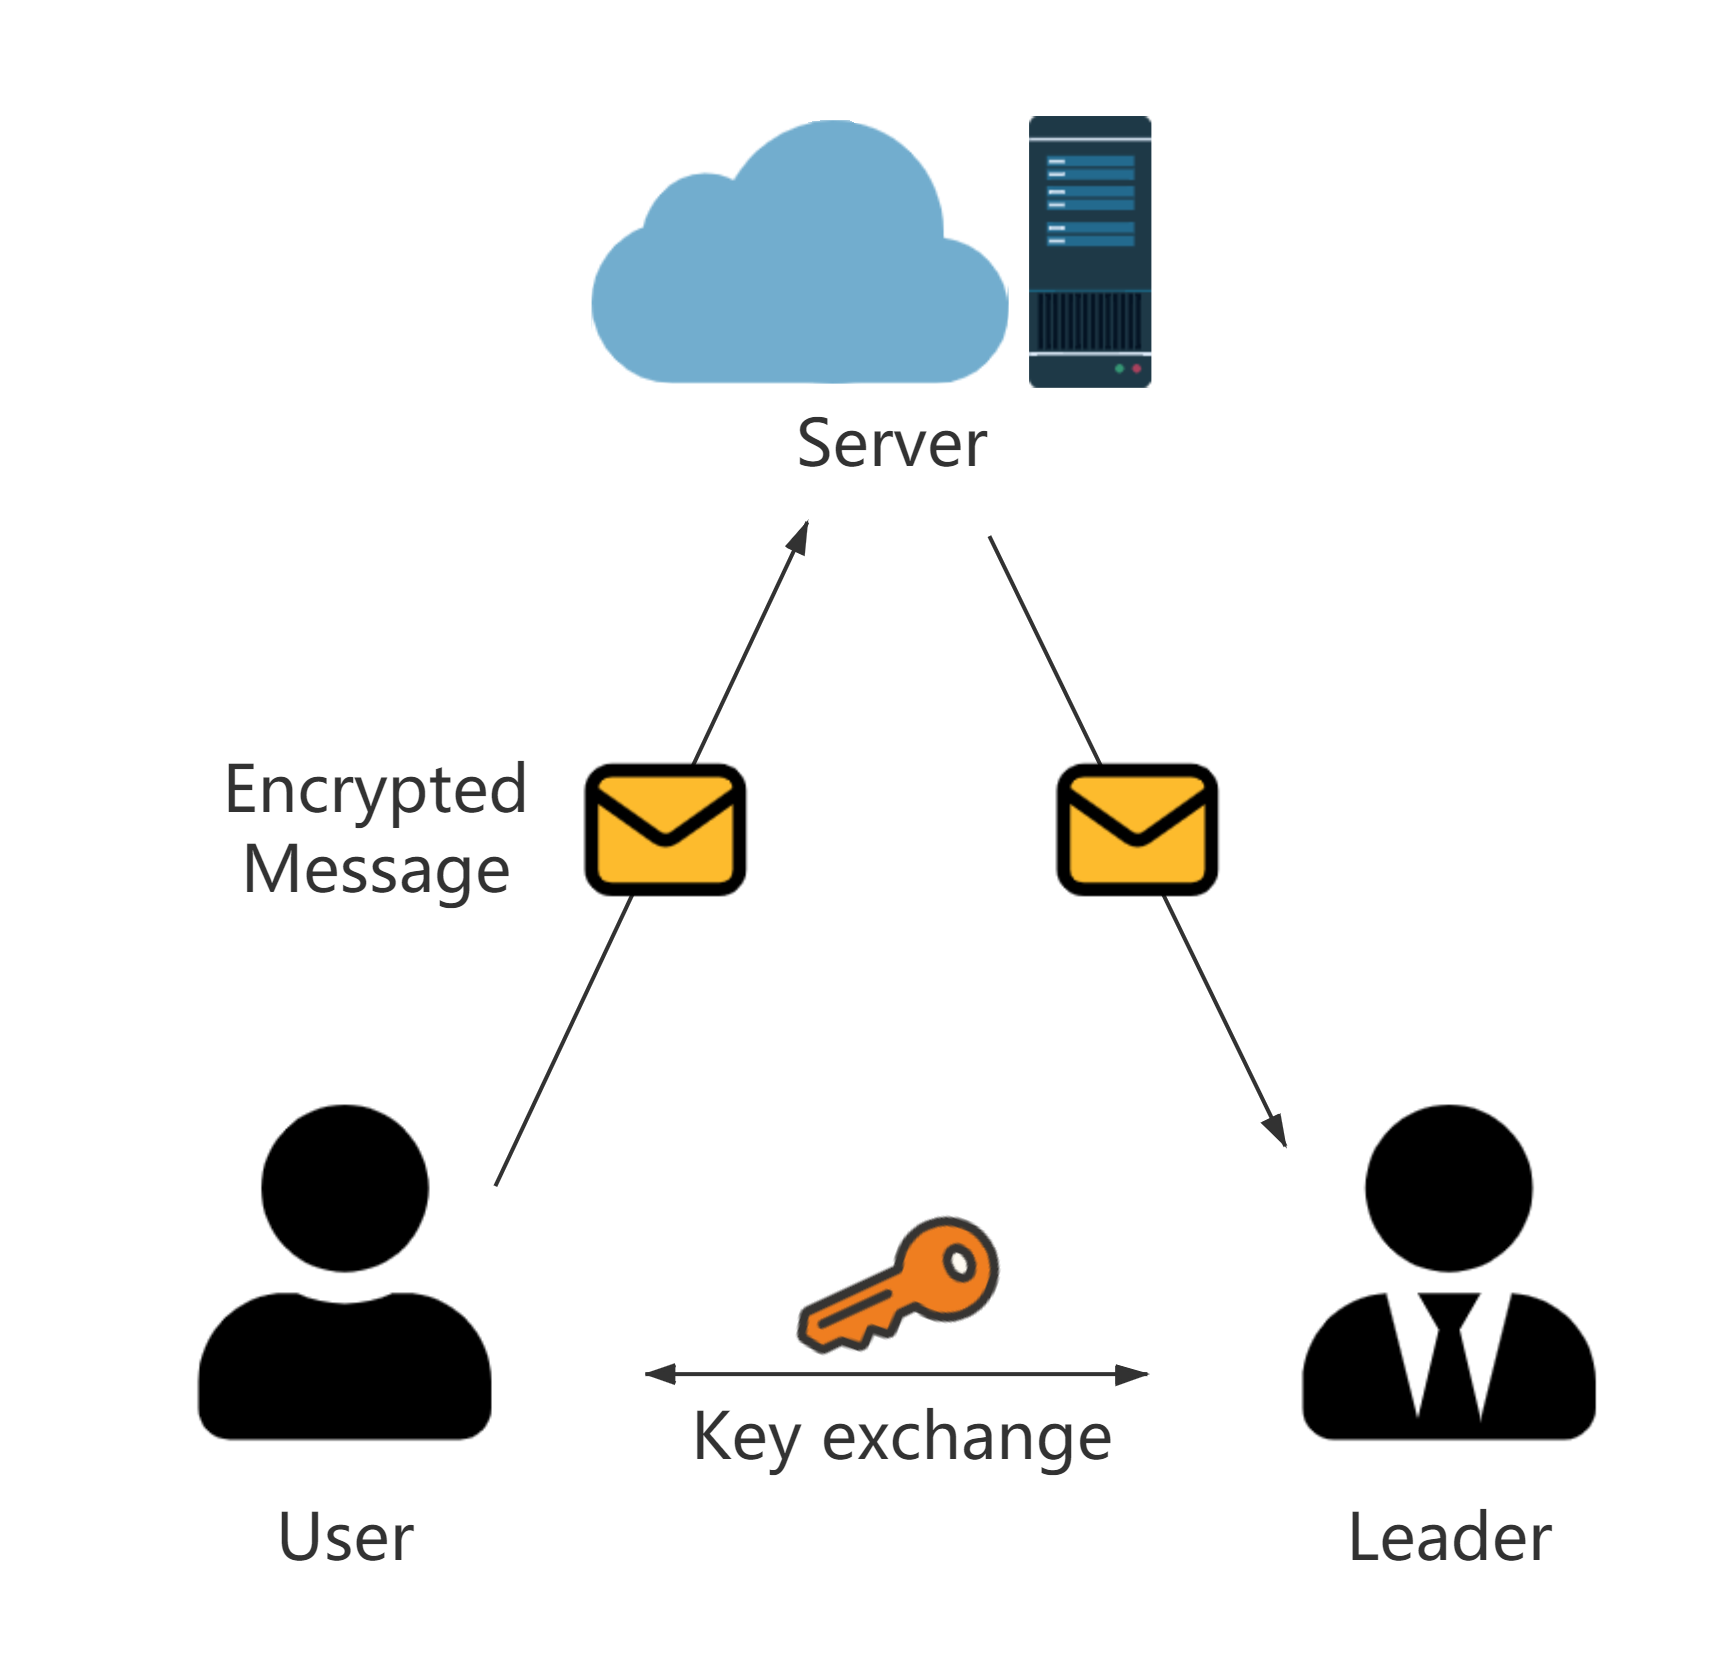
\includegraphics[width=\columnwidth]{img/leader-user.png}
    \caption{The institution can communicate with all users directly while all the leader-user pair share a secret key used for private communication. The server helps to forward encrypted messages from which it can know nothing.}
    \label{leader-user}
\end{figure}

\subsubsection{\textbf{Key exchange}}
When the parties receive $L$, they will know who the leaders are. In order to communicate with the leaders privately, the parties need to run key-exchange protocols to share secret keys. We employ Diffie-Hellman protocol~\cite{DH} to realize it. 
% Google has experimented with DH in federated learning~\cite{Practical} and there are some techniques to improve the performance, which our framework will also adopt.

In a server-based environment, a server can communicate with any clients while the parties are unfamiliar with each other. Therefore, the key exchange process should be conducted in virtue of the server. In the premise that the server is honest-but-curious, parties can exchange keys in a ``man-in-the-middle'' scheme, where the ``man'' is the honest server. The server delivers information for users to help them complete DH protocol. This process is secure because information leaked to the server in key-exchange protocols is useless.

After the key exchange process, each party-leader pair, a party $P_i$ with a leader $L_j$ will share a secret key $K_{ij}$. By means of $K_{ij}$ the party $P_i$ and leader $L_j$ can encrypt their data against the honest-but-curious attacker. The message $m$ can be encrypted as $Enc_{K_{ij}}(m)$. Figure~\ref{leader-user} illustrates the institution-leader-user structure. Normally, the institution and the common users only need to communicate with the leaders.

\subsubsection{\textbf{Secure learning}}
The aggregation algorithm is the same as FedAvg~\cite{mcmahan2016communicationefficient}. A secure multi-party addition protocol is used to realize privacy-preserving. There are $N_l$ leaders in the system. Without loss of generality, we suppose $N_l = 3$. The flow chart of secure learning process is shown in Figure~\ref{fig-alg} and the process is illustrated as below:

\begin{enumerate}
    \item All the selected parties train the model locally. And a party $P_i$ will get a parameter $G_i$.
    
    \item Each $G_i$ is divided into 3 pieces $G_i^1$, $G_i^2$ and $G_i^3$, where $G_i = G_i^1 + G_i^2 + G_i^3$. Then $G_i^j$ is sent to the $j^{th}$ leader $L_j$ respectively.
    
    \item A leader $L_j$ will record a set $B_j$, which consists of the parties that have sent messages to $L_j$. When all the parties' parameters are sent or time is up, the leaders will send all $B_j$ to the server and the server will compute the intersection as $B$. Then $B$ is sent back to all leaders. Each leader reserve parameter shares according to $B$ in case that some parties did not send parameter pieces to all leaders successfully. Parties not included in the intersection are then removed. 

    \item Leader $L_j$ then computes the sum of the parameters:
    $$A_j = \sum_{i=1}^nG_i^j$$ 
    Afterwards, $A_j$ will be sent to the server.

    \item The server computes: 
    $$W_{global} = \frac{A_1 + A_2 + A_3}{C}  = \frac{\sum_{i=1}^nG_i}{C} $$ 
    and it is the target of FedAvg algorithm. $W_{global}$ is used to update the global model and the server will prepare for the next learning round.
\end{enumerate}

$C$ can be obtained in the same manner: replace $G_i$ with $C_i$ and the server can get $C$ privately. In fact, $C_i$ and $G_i$ are sent to leaders at the same time. Alternatively, $C_i$s can also be directly sent to the server without encrypted since they do not help attackers understanding the parameters. When the system decides to discard a party $P_i$ due to $B$, it also needs to discard $C_i$, which will change the amount of training data $C$. The pseudocode of secure learning is illustrated in Algorithm ~\ref{sec-learning}. Neither the server nor any leader can figure out what exactly a certain party's parameter is based on the information it can receive. 

\begin{figure*}[!ht]
    \centering
    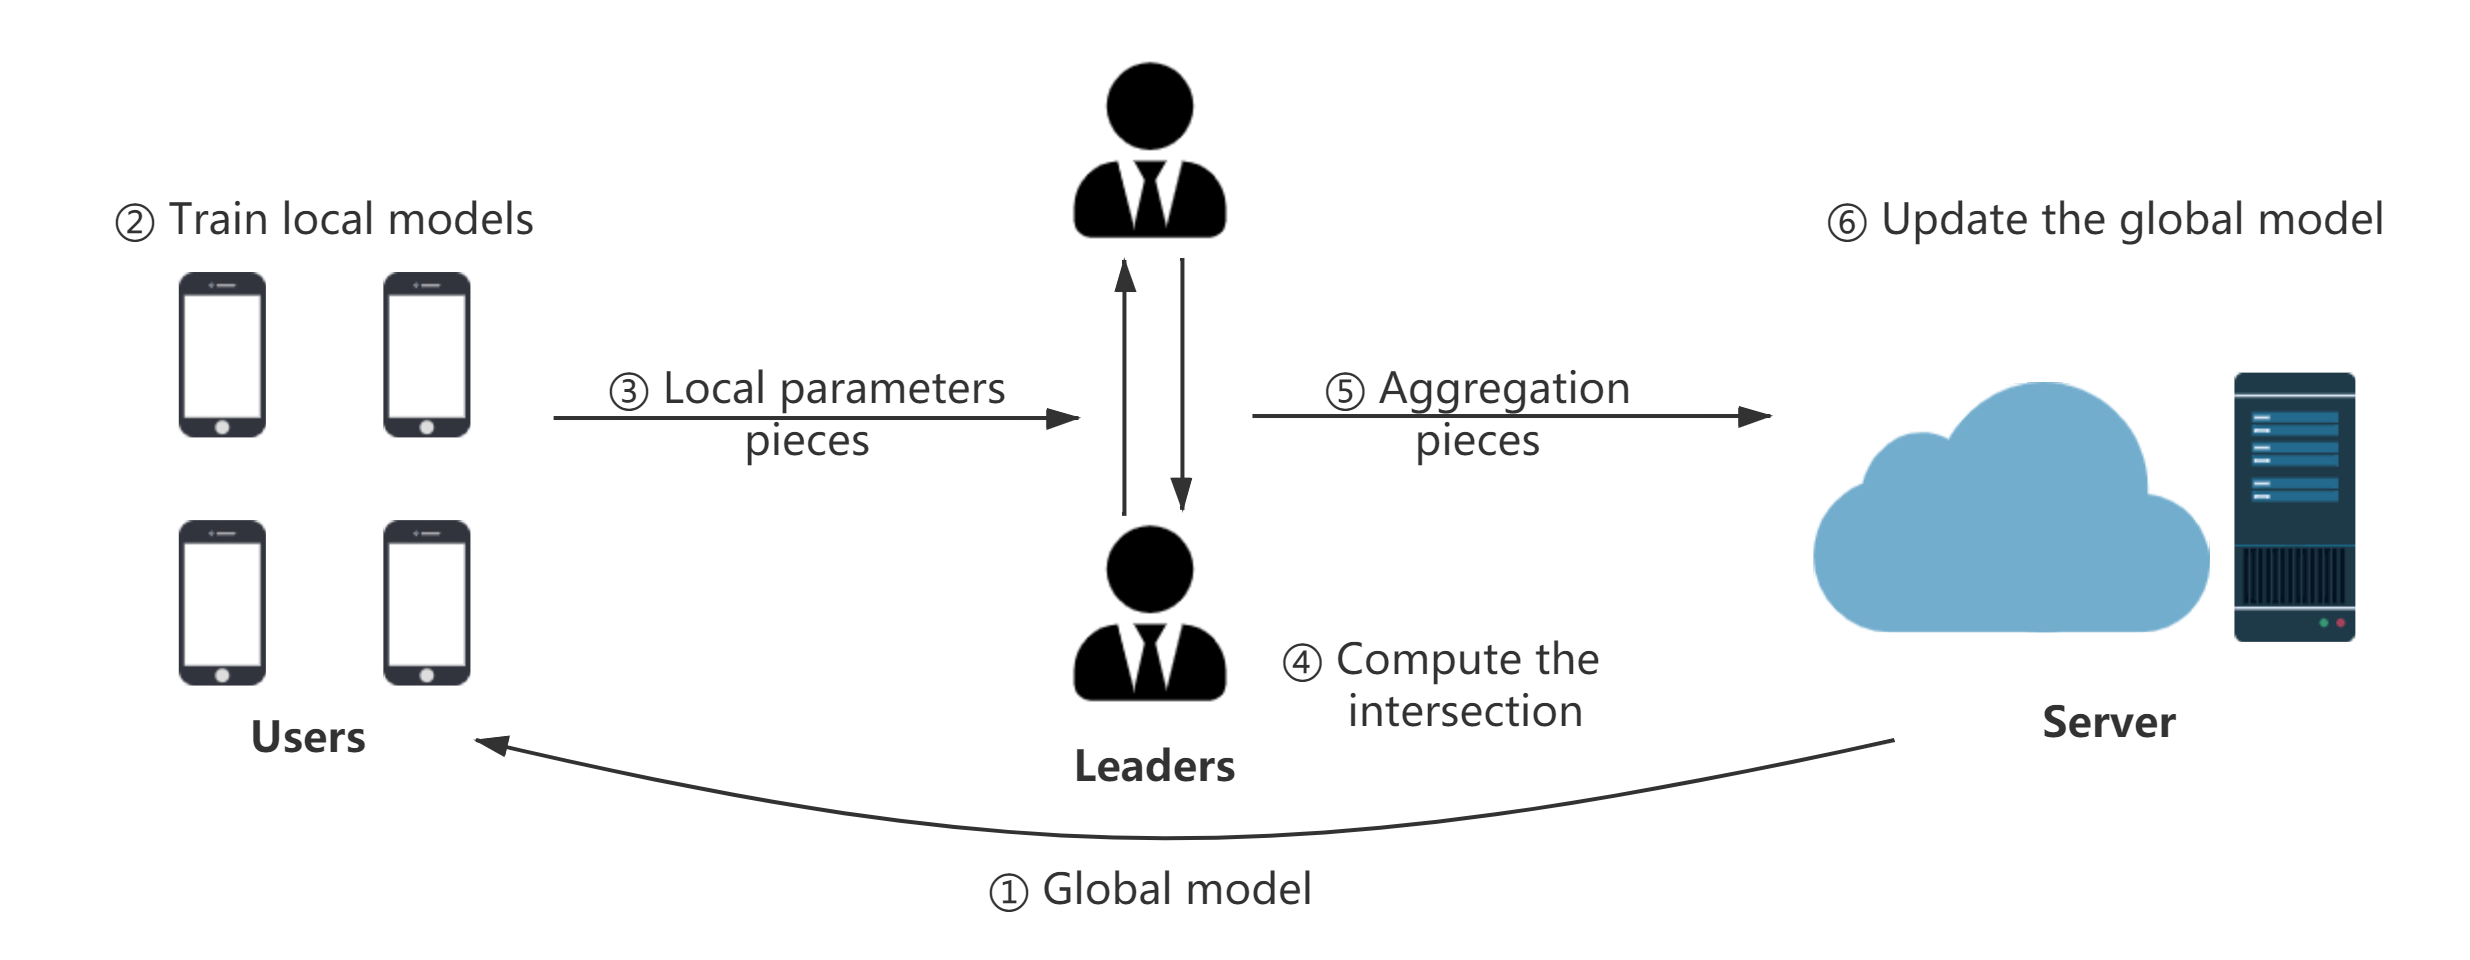
\includegraphics[width=2\columnwidth]{img/alg.png}
    \caption{The flow chart of the secure learning process. It is based on the fact that common users have already constructed secure communication channels with leaders. After step 6, the process will enter the next epoch and restart from step 1.}
    \label{fig-alg}
\end{figure*}

\begin{algorithm}
    \label{sec-learning}
    \caption{Secure Learning Algorithm}
    \begin{algorithmic}[1] 
        \Require $G_i$, $L$, $K_i$ (the set of secret keys for party $P_i$), $E_{max}$ (the maximum epoch for federated learning)
        \Function {split\_parameter}{$G_i$}
            \State $r \gets \Call{random}{0, 0.5}$
            \State $G_i^1 \gets G_i * r$
            \State $r \gets \Call{random}{0, 1-r}$
            \State $G_i^2 \gets G_i * r$
            \State $G_i^3 \gets G_i - G_i^1 - G_i^2$
            \State \Return{$G_i^1, G_i^2, G_i^3$}
        \EndFunction
        \State
        \Function {party\_send}{$G_i, L, K_i$}
            \State $G_i^1, G_i^2, G_i^3 \gets$ \Call{split\_parameter}{$G_i$}
            \For {$j \in$ indexes of $L$}
                \State $E_{ij} \gets \Call{Enc}{K_{ij}, G_i^j}$
                \If {Sends $E_{ij}$ to $L_j$ not successfully}
                    \State Report ``$L_j$ is crashed'' to $S$
                \EndIf
            \EndFor
        \EndFunction
        \State
        \Function {leader\_send}{$K_j$}
            \State $B_j \gets \emptyset$
            \State Receive $E_{ij}$s from all possible $P_i$ and add $i$ to $B_j$
            \State Send $B_j$ to $S$
            \State Receive $B$ from $S$
            \State Remove $E_{ij}$s whose $i$ is not included in $B$
            \State $G_i^j \gets \Call{Dec}{K_{ij}, E_{ij}}$ for each $E_{ij}$
            \State $A_j \gets \sum_{i=1}^nG_i^j$
            \State Sends $A_j$ to $S$
        \EndFunction
        \State
        \Function {server\_aggregation}{e}
            \If{$e \ge E_{max}$}
                \State \Return{$True$}
            \EndIf
            \State Receive $A_j$s from leaders
            \State $W_{global} \gets \frac{A_1 + A_2 + A_3}{C} $
            \State \Call{Update}{$Model_{global}, W_{global}$} 
            \State $//$ Next epoch
            \State Select $n$ parties to participate in the next epoch
            \State Send $W_{global}$ to these $n$ parties
            \State \Return{\Call{server\_aggregation}{e+1}}
        \EndFunction
    \end{algorithmic}
\end{algorithm}


\subsubsection{\textbf{Reorganization}}
The reorganization process provides the robustness for the framework. Normally, the server will notice a leader's crash within a heart-beat cycle. Meanwhile, a party will report to the server if it finds a leader is crashed. After noticing a leader is crashed, the server sends ``stop'' signals to all parties, which will stop the learning processes. Then all parties will perform an election campaign according to the simplified consensus algorithm: they send ``competition'' signals to the server. The server will receive numerous signals and the first one to arrive will be selected as the new leader. $L$ will be updated and sent to all common parties. Finally, the learning process will be restarted.

\subsection{Among-institutions Model}
Since secure P2P communication is already constructed, the key exchange process is removed in this situation. In addition, consensus algorithms can be executed naturally in such an environment as it is in a decentralized system where parties are equal. Therefore, leaders are elected by voting as the original Raft does. The leader-tenure and reorganization processes also vote for new leaders instead of getting leaders from a server.

\section{Efficiency and Security Evaluation}
\label{sec:eval}
\subsection{Communications}
As illustrated in Section III, our framework only adopts simple algorithms to enhance security. Therefore, the execution overhead can be ignored compared to the communication overhead. Notice that any communication in our framework goes through the server. E.g., if $P_i$ wants to send encrypted message $c$ to $L_j$, $c$ will be sent to server $S$ first. Afterwards $S$ will forward $c$ to $L_j$. In general, our P2P communications are emulated with client/server communications. This method accelerates communication greatly because it costs much for two strangers to exchange messages directly. E.g., if two parties want to communicate directly, both of them need to store the addresses, confirm the ``accept'' signal after each message-exchange, et al. However, with a powerful server helping to forward, these things are no longer concerns for parties.

In each round, there are $n$ common parties and $N_l$ leaders. W.l.o.g., we suppose there is no common party that is also a leader at the same time. Common parties, leaders together with the server $S$ are all parties requiring communication. Generally, $N_l$ is a very small number such as 3, therefore we can treat it as a constant number. Our framework can be categorized into \textbf{set-up} and \textbf{epoch-learning} two phases. We analyze these two phases respectively:

\begin{itemize}
    \item \textbf{Set-up:} All $N-N_l$ parties need to construct secure channels with all $N_l$ leaders. Suppose it needs $D$ communications in each DH protocol, then the amount of communications of the set-up phase is $D * (N-N_l) * N_l$. The time complexity is $O(N)$ based on the fact that $D$ and $N_l$ are small constant numbers.
    
    In the re-organization process, $S$ chooses a new leader that needs to conduct DH protocols with all $N-N_l$ parties, which is $D * (N-N_l)$ communications. Therefore, a re-organization process also costs $O(N)$ communications.
    
    \item \textbf{Epoch-learning:} In each epoch, $S$ sends the current $W_{global}$ to $n$ parties, which cost $n$ communications. Then every common party sends $W_{ij}$ to $N_l$ leaders respectively, which cost $n * N_l$ communications. Finally leaders send $Aj$s to $S$, which cost $N_l$ communications. Thus the total cost of one epoch is $n + n * N_l + N_l$, which is $O(n)$.
\end{itemize}

In the time complexity aspect, our framework does not result in higher overhead expect for an $O(N)$ preprocessing compared to the original FedAvg algorithm. In the vertical aspect, our framework does not require more message-exchanges for any party-leader pair. 

\subsection{Security Evaluation}
The evaluation is based on the fact that our adversaries are all honest-but-curious. Since our framework is based on MPC researches~\cite{Shamir,Du2001SecureMC,Three-Party}, the security against message-leakage can be guaranteed. The riskiest threat is the collusion attack. Colluding with a common party has no contribution to an attack because it lets out nothing but the information about this common party, which belongs to the attacker side. Therefore, we only discuss situations that collusion among leaders. 

Apparently, the attacker must collude with all leaders in order to reconstruct one party's parameter. Since the leaders are assigned by the server randomly, it is hardly possible for all attackers to be elected as leaders with the server being honest. However, it is necessary to discuss the situation where the server cheats to select leaders as its wish, though it does not deviate from the learning protocols. In such situations, the leaders are always selected by the unreliable server. To address this problem, we introduced leader-tenure in Section III, which forces the system to change leaders regularly. Since it needs all leaders' betrayal to attack successfully, the system only needs to change one leader regularly. Changing one leader is equivalent to a re-organization process, which cost $O(N)$ time. Therefore, our framework has high security against collusive honest-but-curious attackers.


\section{Experimental Results}
\label{sec:exp}
\subsection{Implementation}
Our framework is implemented with Pytorch. We used AES-GCM-128 as the authenticated encryption algorithm as Bonawitz et al. did~\cite{Practical}. We adopted Mnist and Cifar10 as datasets, which are also used in the original FedAvg~\cite{mcmahan2016communicationefficient}. We trained simple convolutional neural networks for the classification task. Our experiments are carried on a PC with an Intel i7-8700 CPU (3.2GHz), 16 GB of RAM, and a GTX 1080 GPU. The model was executed in a single thread to facilitate comparing and analyzing. The optimizer was stochastic gradient descent (SGD) and the learning rate is $0.01$. The $fraction$ is set as $0.1$ which means that $10\%$ of clients will be chosen to carry on the training process in each epoch. 
% Our demo is open-sourced on \url{https://github.com/Carudy/sofl}.


\subsection{Accuracy}
Although our work does not modify the learning module compared to other federated learning frameworks, we still conducted a series of experiments to observe the accuracy. We compared FedAvg with our framework on both independently identically distribution (iid) data and non-iid data to verify the effectivity. Since this experiment aims to prove the validity instead of high accuracy, the models were not trained to high accuracy. Figure~\ref{acc} shows the result. With iid data, our framework obtains accuracy quite similar to FedAvg. With non-iid data, the two systems did not match as well as they were with iid data when the $epoch$ was small. However, they finally converged to the same stable scope with the same speed, which confirmed the differences were caused by biases. Therefore, our framework changes nothing about federated learning and it only provides privacy and robustness. 

\begin{figure}[!ht]
    \centering
    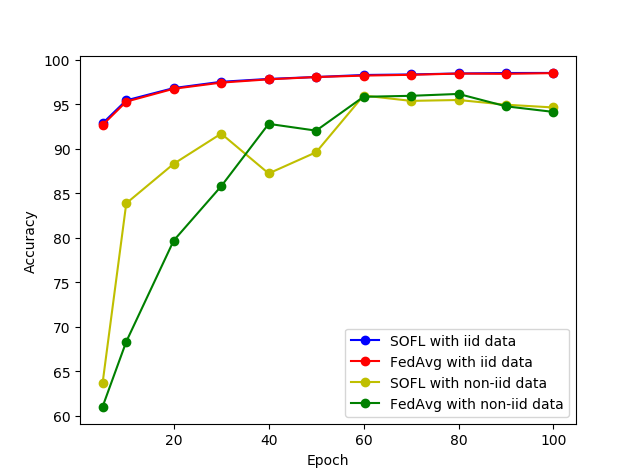
\includegraphics[width=\columnwidth]{img/acc.png}
    \caption{The accuracy of FedAvg and SOFL with iid and non-iid data in MNIST dataset. The horizontal axis $epoch$ means the total rounds that the federated learning system has been trained for.}
    \label{acc}
\end{figure}

\begin{figure}[!ht]
    \centering
    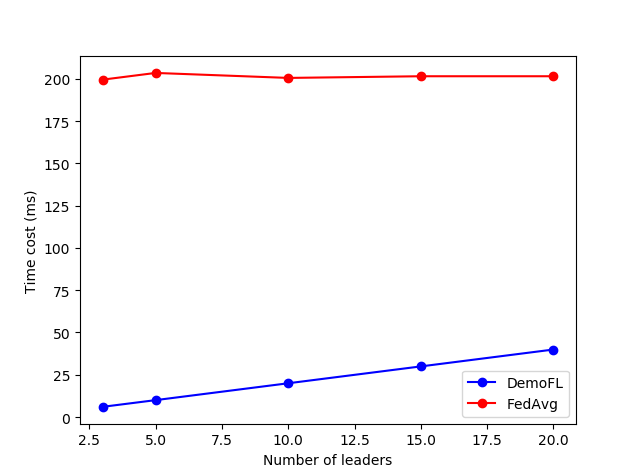
\includegraphics[width=\columnwidth]{img/leader-time.png}
    \caption{Total time spent on computation for DH protocols of Bonawitz's FedAvg~\cite{Practical} and SOFL. The number of clients is set as 100.}
    \label{leader-time}
\end{figure}

\subsection{Set-up Overhead}
In the set-up phase, our system selects several clients as leaders, and the number of leaders impacts the efficiency and a particular leader's load. We set the number of clients as $100$, and Figure~\ref{leader-time} shows the linear relation between computation time spent on Diffie Hellman key-exchange protocols and the number of leaders. The time spent on computation for DH protocols can be ignored compared to the learning process due to its low cost.

Meanwhile, with more leaders, one common client needs to store more keys for leaders. Apparently, the relationship between the number of leaders and one client's storage overhead is also linear. In addition, we can consider that in the key-exchange process of Bonawitz et al.~\cite{Practical}'s system, all common clients are leaders, which requires all client-pairs to exchange keys and results in high overhead. The set-up overhead is also illustrated in Figure~\ref{leader-time}. Since it has no leaders, the computation cost does not change. Method of Kanagavelu et al.~\cite{Two-Phase} performs the same as FedAvg because they did not take advantage of the server. Therefore, employing fewer leaders can help to improve efficiency. In contrast, employing more leaders can are beneficial to robustness because it is more flexible for t-out-of-n secret sharing methods, which we will discuss later. 


\subsection{Efficiency}
As introduced before, the additional computation insignificant compared to the communication overhead. Since the communication cost varies with equipment and environments, it is more sufficient to measure the overhead using the number of communications instead of wall clock time. Note that communication in our simulation means two communications in practice: a client needs to send a message to the server first, and the server forwards the message to the corresponding leader. We fixed the number of leaders to 3. The amount of communications increases with the $epoch$, and the result is displayed in Figure~\ref{comm-epoch} with the assumption that there is no dropout of packets. The number of clients is another factor that impacts efficiency. We conducted experiments with the $epoch$ set to 30 and got the results shown in Figure~\ref{comm-client}. The result is the same as what we analyzed in Section IV, which means they are all of the linear time complexity. Although the number of leaders also has an influence on the number of communications, we did not conduct corresponding experiments because it is always set as a very small number. 


\begin{figure}[!ht]
    \centering
    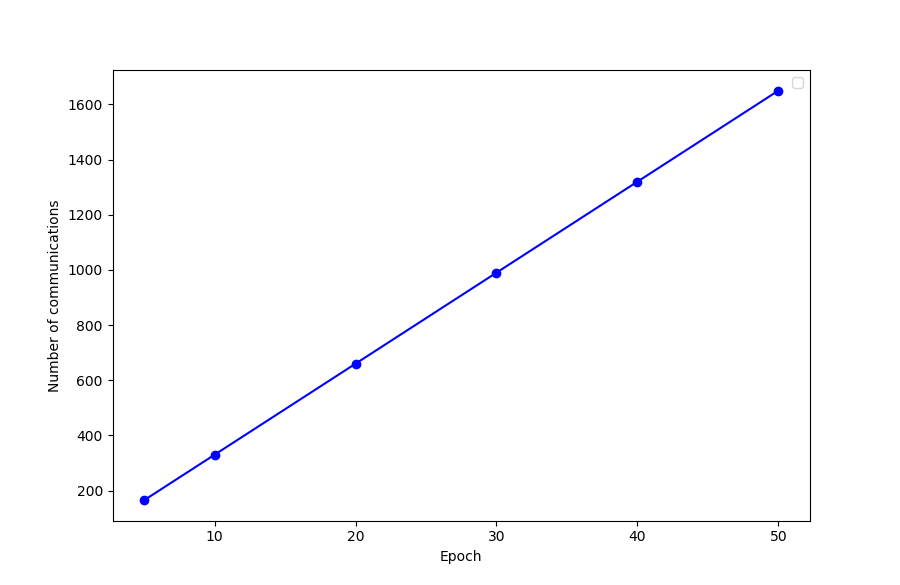
\includegraphics[width=\columnwidth]{img/comm-epoch.png}
    \caption{The amount of communications in learning process with 100 clients without dropout.}
    \label{comm-epoch}
\end{figure}

\begin{figure}[!ht]
    \centering
    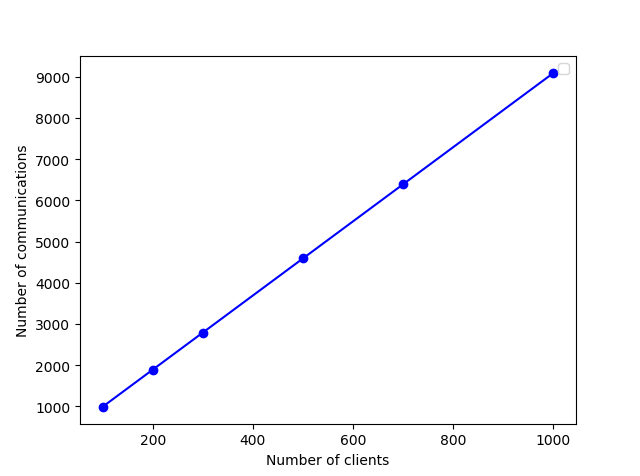
\includegraphics[width=\columnwidth]{img/comm-client.png}
    \caption{The amount of communications in learning process varies VS  the amount of clients. The $Epoch_{max}$ is fixed to 30 and there is no dropout.}
    \label{comm-client}
\end{figure}


\subsection{Robustness}
\subsubsection{Crash}
The robustness of SOFL is mainly based on the re-organizing process, which happens when a leader is crashed. Crashes can hardly be completely avoided, therefore, we introduced $crash\_rate$, which is the possibility that a leader would crash during one epoch, to help to measure the robustness. Generally, we consider $crash\_rate$ is quite small because real crashes rarely happen in nowadays smart devices/servers. However, compared to real crashes, a leader is more likely to be unavailable due to various reasons, which also seldom happen. Therefore we still consider $crash\_rate$ would not be larger than $0.1$. We conducted several experiments on how $crash\_rate$ impacts efficiency. First, we set the number of clients to 100 and the $Epoch_{max}$ to 10. Figure~\ref{comm-crash} shows that when crashes happened, it impacts the same on the value of communications instead of the ratio despite the $epoch$. E.g., a crash with $epoch$ 10 resulted in $66\%$ overhead approximately, and it only resulted in about $0.06\%$ overhead when the $epoch$ is $100$. It indicates that a high $crash\_rate$ does impact the efficiency heavily when $epoch$ is low. However, when the $epoch$ gets larger, the influence of crashes becomes insignificant. Considering that the $epoch$s used in real federated learning works are quite large, SOFL provides sufficient efficiency and robustness.

\begin{figure}[!ht]
    \centering
    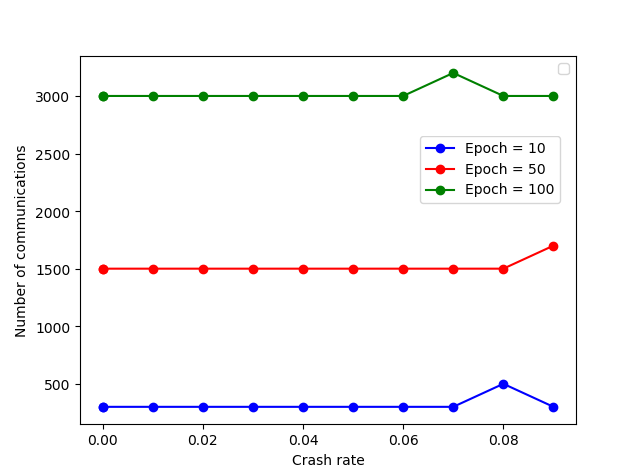
\includegraphics[width=\columnwidth]{img/comm-crash.png}
    \caption{The average amount of communications VS different crash rates.}
    \label{comm-crash}
\end{figure}

\begin{figure}[!ht]
    \centering
    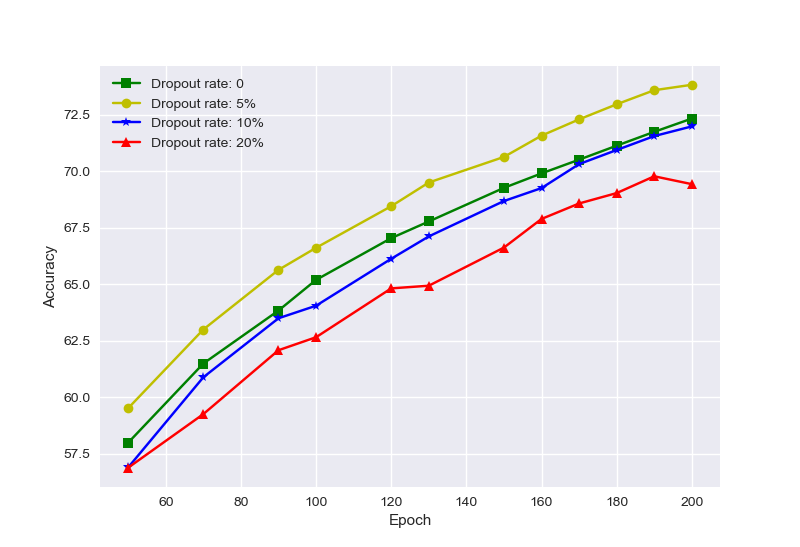
\includegraphics[width=\columnwidth]{img/dropout-acc.png}
    \caption{The average amount of communications VS different dropout rates.}
    \label{dropout-acc}
\end{figure}

\subsubsection{Network Delay and Dropout}
Sometimes several packets cannot be received in time due to network delays or dropouts. Bonawitz et al.'s method~\cite{Practical} has considered this issue and it has a pseudorandom generator (PRG) based masking algorithm to solve it, which has a high computation overhead. In SOFL's secure learning process, a leader will not be waiting for participants'parameters permanently. It has a time limit, over which the leader will abandon waiting and send the current $B_j$ to the server (introduced in Section~\ref{sec:sofl}). Under this circumstance, some common parties will be recognized as having lost connection and removed from the participant-group without contributing to the learning process. However, if a party does not lose the connection while its message reached the leader late because of network delay, discarding it may influence the learning speed and result. We set the dropout rate to show the probability that a common party fails to send its parameters to leaders due to packet loss or network delay. Therefore, we carried out several experiments to observe how network delay impacts the learning process. The result is shown in Figure~\ref{dropout-acc}. We observed that the influence of dropouts on accuracy becomes trivial as the learning process goes on. The accuracy is reduced by only 0.002 in the worst case, which may be caused by biases. Therefore, SOFL has a strong resistance to packet loss. 

\section{Conclusion and Future Works}
\label{sec:conc}
In this paper, we proposed a novel, efficient and privacy-preserving federated learning framework named Self-organizing Federated Learning (SOFL). SOFL adopted MPC-based secret sharing methods to achieve privacy-preserving against honest-but-curious adversarials. It also employs consensus algorithms based leader election algorithms to reduce the communication cost and provide higher efficiency and robustness. Our experiments showed that SOFL has a linear time complexity VS either number of clients or training rounds. And it has a high resistance to member changes. SOFL is lightweight and easy-deploying for many existing federated frameworks such as Pysyft and FATE.

However, it still remains a problem for federated learning that malicious attackers are more harmful and difficult to defend against compared to honest-but-curious attackers. A malicious attacker can deviate from designed protocols or cheat on data that would go through it. Enhanced MPC protocols such like SPDZ\cite{SPDZ} may help dealing with malicious attackers, which could be a future work. Therefore, detecting malicious nodes is a challenging work. In addition, other federated learning schemes besides FedAvg may contain algebraic calculus more than only addition and multiplication, which means existing MPC based methods will gain high overhead on those schemes. Some blockchain techniques are inspiring to solve the malicious attacks such as poisoning and adversarial examples, which may be adopted to enhance SOFL to provide higher security by preventing frauds. It would be significative and interesting for a future work to find more approaches about improving the security and efficiency of federated learning.


\bibliography{main.bib}
\bibliographystyle{IEEEtran}
\end{document}